\documentclass{article}
\usepackage[a4paper, hmargin={2.8cm, 2.8cm}, vmargin={2.5cm, 2.5cm}]{geometry}
\usepackage{eso-pic} % \AddToShipoutPicture
\usepackage{graphicx} % \includegraphics

% Pakker til skrifttyper, tekst osv.
% %%%%%%%%%%%%%%%%%%%%%%%%%%%%%%%%%%%%%%%%%%%%%%%%%%%%%%%%%%%%%%%%%%%%%%%%%%%%%
    \usepackage[utf8]{inputenc} % Implementere Unicode
    \usepackage[T1]{fontenc}    % Unicode skrifttype, fx. é skrives som 1 tegn
 %    \usepackage[english]{babel} % Engelsk Ordbog
   \usepackage[danish]{babel}  % Dansk Ordbog
    \usepackage{microtype}      % Forbedre linjeombrydningen
    \usepackage{libertine}      % Skrifttype
    \usepackage[scaled=0.83]{inconsolata} % Skrifttype til kode til kode
% %%%%%%%%%%%%%%%%%%%%%%%%%%%%%%%%%%%%%%%%%%%%%%%%%%%%%%%%%%%%%%%%%%%%%%%%%%%%%


% Pakker til matematik og kode.
% %%%%%%%%%%%%%%%%%%%%%%%%%%%%%%%%%%%%%%%%%%%%%%%%%%%%%%%%%%%%%%%%%%%%%%%%%%%%%
    \usepackage{mathtools}       % Udvidelse til amsmath pakken
    \usepackage{algpseudocode}   % pseudocode til algoritmer
    \usepackage{algorithm}       % Pakke til algoritmer
    \usepackage{amsthm}          % Pakke til Theroms
% %%%%%%%%%%%%%%%%%%%%%%%%%%%%%%%%%%%%%%%%%%%%%%%%%%%%%%%%%%%%%%%%%%%%%%%%%%%%%

% Pakker til layout.
% %%%%%%%%%%%%%%%%%%%%%%%%%%%%%%%%%%%%%%%%%%%%%%%%%%%%%%%%%%%%%%%%%%%%%%%%%%%%%
    \usepackage{fancyhdr}        % Gør det muligt at bruge sidehoveder
    \usepackage{graphicx}        % Mulighed for bl.a. \includegraphics
    \usepackage{colortbl}        % Hvis man vil farvelægge sine tabeller
    \usepackage{array}           % Gør miljøerne array og tabular lidt bedre
    \usepackage{parskip}         % Første paragraf i afsnit indrykkes ikke
    \usepackage{listings}        % Pakke til at indsætte kode
    \usepackage{enumitem}        % Gør det muligt at tilpasse lister
    \usepackage{titlesec}        % Tilpassing af afstand mellem sektioner
    \usepackage[lastpage,user]{zref} % Side x af y
% %%%%%%%%%%%%%%%%%%%%%%%%%%%%%%%%%%%%%%%%%%%%%%%%%%%%%%%%%%%%%%%%%%%%%%%%%%%%%


% Ikke standard pakker
% %%%%%%%%%%%%%%%%%%%%%%%%%%%%%%%%%%%%%%%%%%%%%%%%%%%%%%%%%%%%%%%%%%%%%%%%%%%%%
%    \usepackage{boxproof}        % Til at lave bevis kasser i logik
    %\usepackage{semantic}        % Pakke til logik med ->, |- osv.
%    \usepackage{daymonthyear}    % Giver info om dato.
% %%%%%%%%%%%%%%%%%%%%%%%%%%%%%%%%%%%%%%%%%%%%%%%%%%%%%%%%%%%%%%%%%%%%%%%%%%%%%


% Implementere en række makroer og de pakker der er importeret
% %%%%%%%%%%%%%%%%%%%%%%%%%%%%%%%%%%%%%%%%%%%%%%%%%%%%%%%%%%%%%%%%%%%%%%%%%%%%%
    \pagestyle{fancy}                        % Implementere sidehoved
    \lhead{Københavns Universitet} % Venstre sidehoved
    \rhead{Evaluering af Datalogisk Fagpakke}                      % Højre sidehoved
    \cfoot{\thepage\ of \zpageref{LastPage}} % Side x af y
    \newtheorem*{prp}{Propostion}            % Skaber nyt theorem
    \setlist{nolistsep}                      % Formindsker mellemrum mellem listepunkter


    % Definitioner af farver
    % %%%%%%%%%%%%%%%%%%%%%%%%%%%%%%%%%%%%%%%%%%%%%%%%%%%%%%%%%%%%%%%%%%%%
        \definecolor{KURed1}{RGB}{144,26,30}    % Official KU Red 1
        \definecolor{KURed2}{RGB}{199,36,41}    % Unofficial KU Red
        \definecolor{KUGray1}{RGB}{102,102,102} % Official KU Gray 1
        \definecolor{KUGray2}{RGB}{133,133,133} % Official KU Gray 2
        \definecolor{KUGray3}{RGB}{163,163,163} % Official KU Gray 3
        \definecolor{KUGray4}{RGB}{194,194,194} % Official KU Gray 4
        \definecolor{KUGray5}{RGB}{224,224,224} % Official KU Gray 5
    % %%%%%%%%%%%%%%%%%%%%%%%%%%%%%%%%%%%%%%%%%%%%%%%%%%%%%%%%%%%%%%%%%%%%


    % Mindsker afstanden mellem sektioner
    % %%%%%%%%%%%%%%%%%%%%%%%%%%%%%%%%%%%%%%%%%%%%%%%%%%%%%%%%%%%%%%%%%%%%
        \titlespacing\section{0pt}{12pt plus 4pt minus 2pt}
                                  {0pt plus 1pt minus 3pt}
        \titlespacing\subsection{0pt}{12pt plus 4pt minus 2pt}
                                  {0pt plus 1pt minus 3pt}
        \titlespacing\subsubsection{0pt}{12pt plus 4pt minus 2pt}
                                  {0pt plus 1pt minus 3pt}
    % %%%%%%%%%%%%%%%%%%%%%%%%%%%%%%%%%%%%%%%%%%%%%%%%%%%%%%%%%%%%%%%%%%%%


    % Genveje
    % %%%%%%%%%%%%%%%%%%%%%%%%%%%%%%%%%%%%%%%%%%%%%%%%%%%%%%%%%%%%%%%%%%%%
    \def\meta#1{\mbox{$\langle\hbox{#1}\rangle$}} % Mbox til premiser
    \def\intro#1{{#1}{\cal I}}
    \def\elim#1{{#1}{\cal E}}
    \let\imp\to
    \let\implies\to

    % %%%%%%%%%%%%%%%%%%%%%%%%%%%%%%%%%%%%%%%%%%%%%%%%%%%%%%%%%%%%%%%%%%%%


    % Milø til kode
    % %%%%%%%%%%%%%%%%%%%%%%%%%%%%%%%%%%%%%%%%%%%%%%%%%%%%%%%%%%%%%%%%%%%%
        \lstdefinestyle{kode}{
            basicstyle=\scriptsize\ttfamily\color{black},
            keywordstyle=\bfseries\color{KURed1},
            commentstyle=\bfseries\color{KUGray1},
            identifierstyle=\color{black},
            stringstyle=\color{KURed2},
            breaklines=false,
            showspaces=false,
            showstringspaces=false,
            extendedchars=true,
            breakatwhitespace=false,
        }
        \lstnewenvironment{code}[1][]
        {\minipage{\linewidth}
            \lstset{
                #1,
                style=kode,
                escapeinside={!!}{!!},
                frame=tb,
                }
        }
        {\endminipage}
    % %%%%%%%%%%%%%%%%%%%%%%%%%%%%%%%%%%%%%%%%%%%%%%%%%%%%%%%%%%%%%%%%%%%%


    % Laver titel
    % %%%%%%%%%%%%%%%%%%%%%%%%%%%%%%%%%%%%%%%%%%%%%%%%%%%%%%%%%%%%%%%%%%%%
    \title{
      \vspace{10em}
      \Large{Københavns Universitet} \\
      \Huge{Evaluering af 3-Ugers forløb i Data analyse hos HTX Sukkertoppen}
    }

    \author{
    	 \Large{Arinbjörn Brandsson - Arbr@di.ku.dk }\\
      	\Large{Benjamin Rotendahl - Bero@di.ku.dk}\\
         \Large{Mathias Fleig Mortensen - Mamo@di.ku.dk }
    }

    \date{
        \vspace{25em}
        \today
    }
    % %%%%%%%%%%%%%%%%%%%%%%%%%%%%%%%%%%%%%%%%%%%%%%%%%%%%%%%%%%%%%%%%%%%%

% %%%%%%%%%%%%%%%%%%%%%%%%%%%%%%%%%%%%%%%%%%%%%%%%%%%%%%%%%%%%%%%%%%%%%%%%%%%%%


%%%%%%%%%%%%%%%%%%%%      Her starter documentet    %%%%%%%%%%%%%%%%%%%%%%%%%%%
\begin{document}


    %% Change `ku-farve` to `nat-farve` to use SCIENCE's old colors or
    %% `natbio-farve` to use SCIENCE's new colors and logo.
    \AddToShipoutPicture*{\put(0,0){\includegraphics*[viewport=0 0 700 600]{include/ku-farve}}}
    \AddToShipoutPicture*{\put(0,602){\includegraphics*[viewport=0 600 700 1600]{include/natbio-farve}}}

    %% Change `ku-en` to `nat-en` to use the `Faculty of Science` header
    \AddToShipoutPicture*{\put(0,0){\includegraphics*{include/nat-en}}}

    \clearpage

%Disse linjer skaber forside, evt indholdsfortegnelse, og sætter sidetal
%%%%%%%%%%%%%%%%%%%%%%%%%%%%%%%%%%%%%%%%%%%%%%%%%%%%%%%%%%%%%%%%%%%%%%%%%%%%%
    \maketitle              % Forside
    \thispagestyle{empty}   % Fjerner sidetal forside

        % Slå disse til hvis der ønskes indholdsfortegnelse
        % %%%%%%%%%%%%%%%%%%%%%%%%%%%%%%%%%%%%%%%%%%%%%%%%%%%%%%%%%%%%%%%%%%%%%
            %\newpage                % Side til indholdsfortegnelse
            %\thispagestyle{empty}   % Fjerner sidetal fra indholdsfortegnelse
            %\tableofcontents        % Skaber indholdsfortegnelse
        % %%%%%%%%%%%%%%%%%%%%%%%%%%%%%%%%%%%%%%%%%%%%%%%%%%%%%%%%%%%%%%%%%%%%%

    \newpage                % Første rigtige side
    \setcounter{page}{1}    % Sætter rigtigt sidetal på første side
%%%%%%%%%%%%%%%%%%%%%%%%%%%%%%%%%%%%%%%%%%%%%%%%%%%%%%%%%%%%%%%%%%%%%%%%%%%%%
\section{Introduktion}
    Fra uge 43-45 var vi hver tirsdag ude hos HTX sukkertoppen for at undervise
    to klasser i algoritmer og data analyse.
    I dette dokument præsenteres den evaluering vi bad eleverne om at udfylde.

\section{Evaluering af de individuelle uger}
    \subsection{Uge 1}
    \begin{figure}[h!]
        \centering
        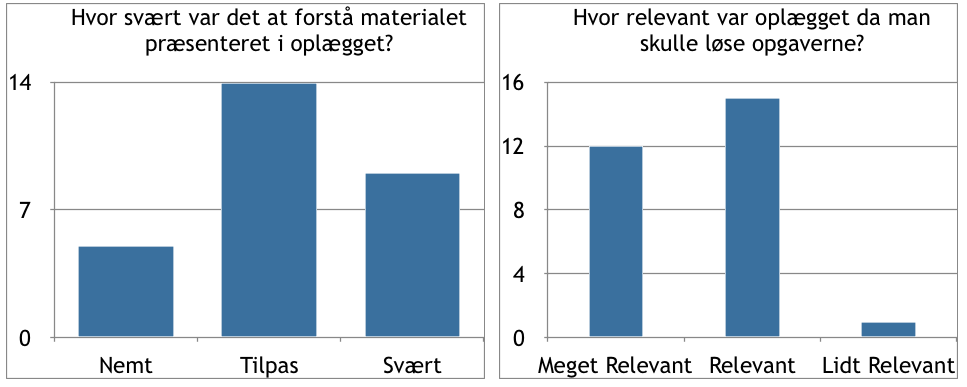
\includegraphics[width=1\textwidth]{include/uge1-1.png}
    \end{figure}

    \begin{figure}[h!]
        \centering
        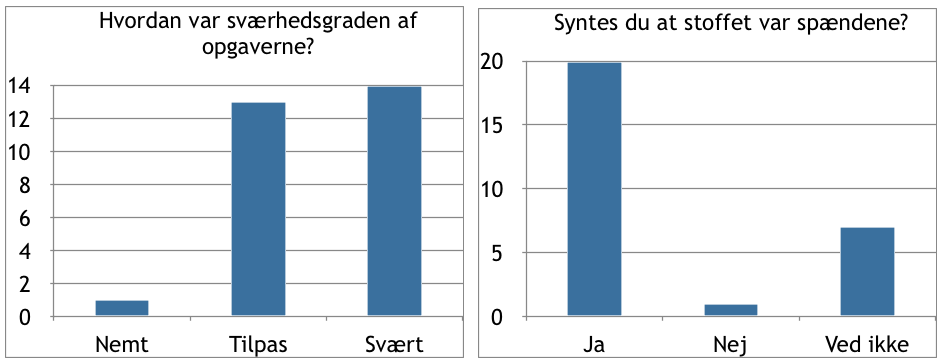
\includegraphics[width=1\textwidth]{include/uge1-2.png}
    \end{figure}

    \subsubsection{Kommentarer til uge 1}
    \begin{itemize}
        \item Var desværre ikke til stede i uge 1

        \item Opgaverne gav god mening, og var underholdene at løse, og nemme
              nok til at de var hurtige, så man ikke sad for lang tid og
              kæmpede, men stadig være nok til at man havde en sejersfølelse når
              man havde lavet dem rigtigt.
        \item Savner pointsystem alá det på UNF
        \item Svært at forstå da det er første gangs øvelser
        \item Det var fedt at se at stoffet kunne formidles på en let og
              overskuelig måde.

        \item "Lærene/de studrende" var meget pædagogiske i deres formidling,
              super godt!

        \item Fed introduktion, der helt klart fangede min interesse.

        \item Jeg synes at det var spændende. Der var dog for kort tid.
    \end{itemize}
\newpage
    \subsection{Uge 2}
    \begin{figure}[h!]
        \centering
        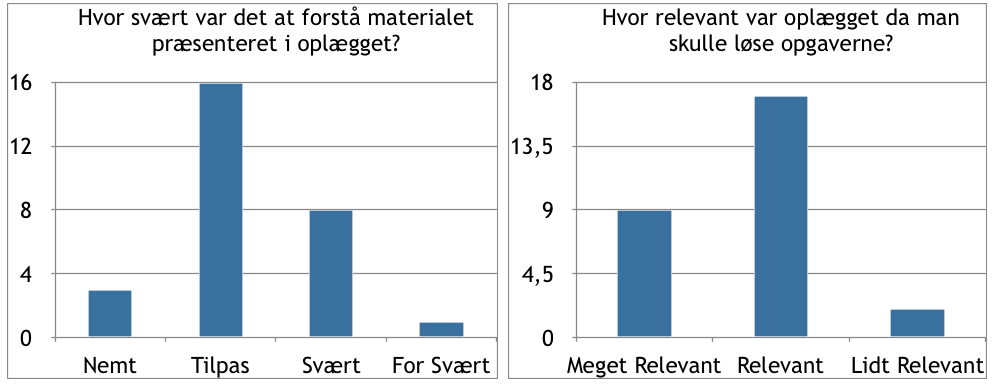
\includegraphics[width=1\textwidth]{include/uge2-1.png}
    \end{figure}

    \begin{figure}[h!]
        \centering
        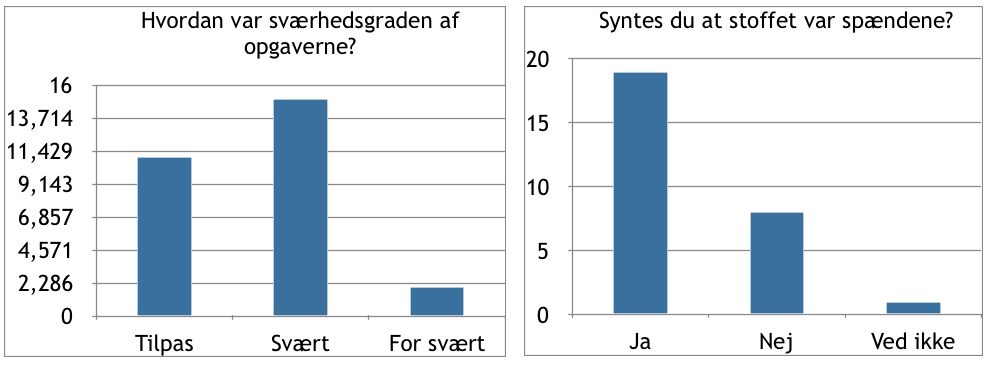
\includegraphics[width=1\textwidth]{include/uge2-2.png}
    \end{figure}
    \vspace{-1em}
    \begin{figure}[h!]
        \centering
        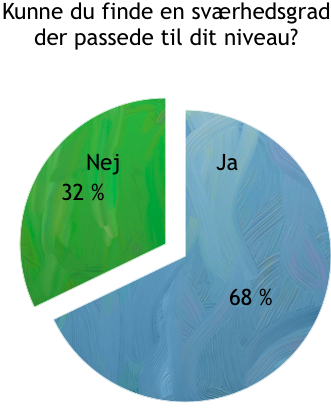
\includegraphics[width=0.3\textwidth]{include/uge2-3.png}
    \end{figure}


    \subsubsection{Kommentarer til uge 2}
    \begin{itemize}
        \item Det ville være fedt hvis man fik svar på om man havde gjort det
              rigtigt eller forkert

        \item Hvis man ikke har forhenværende forståelse for kodning, det være
              meget svært, og meget abstrakt at sætte sig ind i.

        \item Kunne ikke rigtig forstå Python, da jeg syntes det virker bagvendt
              i forhold til andre programmerings sprog, men det er generelt et
              godt sprog at gå til da det var brugervenligt for begyndere.

        \item Var der ikke :P

        \item gøre det nemmere for dem som ikke ved hvad det går ud på og ikke
              kan finde ud af det.

        \item Har selv leget lidt med programmering, men online-kurser er altså
              ikke helt det samme som faktisk undervisning.

        \item Igen synes jeg at det var godt og at der ikke var nok tid.
              Desuden burde vi måske bedes skrive nogle noter til modulet,
              da vi sikkert har glemt, hvad der skete i uge 1 og 2 i uge 3.
    \end{itemize}
\newpage
    \subsection{Uge 3}
    \begin{figure}[h!]
        \centering
        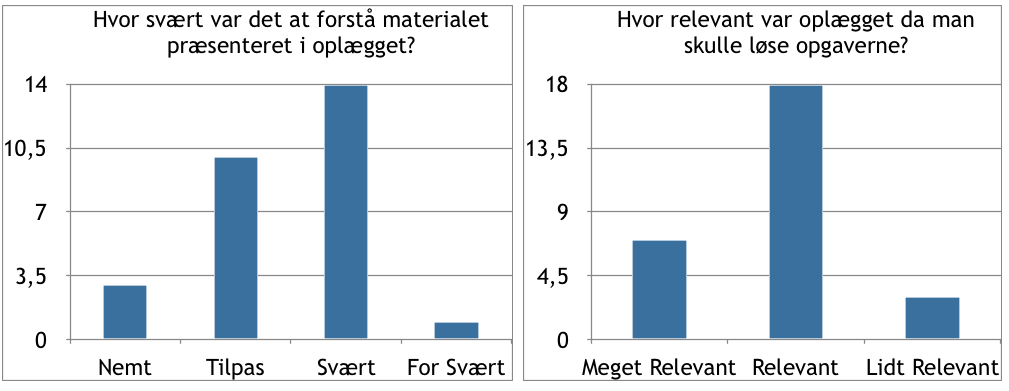
\includegraphics[width=1\textwidth]{include/uge3-1.png}
    \end{figure}

    \begin{figure}[h!]
        \centering
        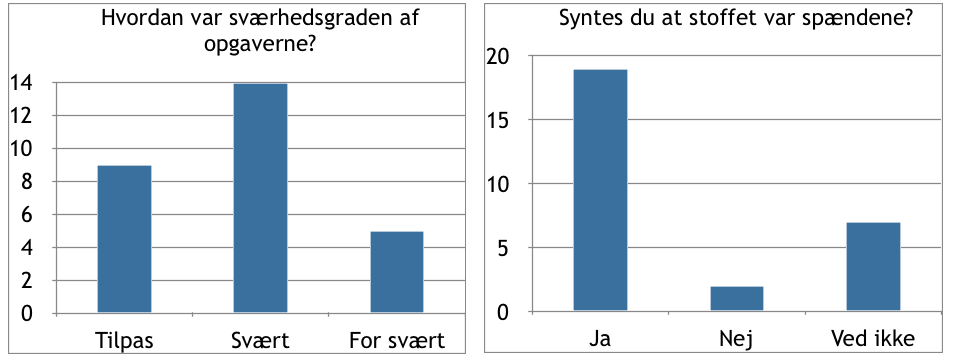
\includegraphics[width=1\textwidth]{include/uge3-2.png}
    \end{figure}

    \begin{figure}[h!]
        \centering
        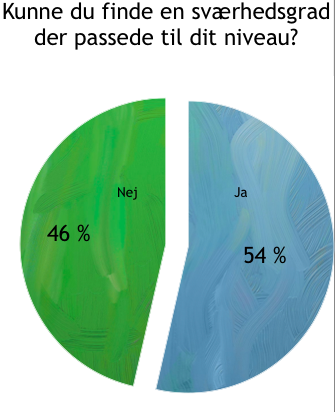
\includegraphics[width=0.3\textwidth]{include/uge3-3.png}
    \end{figure}


    \subsubsection{Kommentarer til uge 3}
    \begin{itemize}
        \item Det ville være fedt hvis man fik svar på om man havde gjort det
              rigtigt eller forkert

        \item Det var spændende, men svært. Synes det var godt at i satte et
              praktisk relevant eksempel på det.

        \item Igen var det svært pga. forståelses problemer, men hvis jeg vidste
              lidt mere om Python ville opgaverne nok være væsentligt nemmere

        \item Det var lidt svært at finde ud af hvad der var hvad og hvad der
              passede ind i hvilke funktioner

        \item Vældig relevant stof. Super spændende og helt klart dér, hvor
              fremtiden ligger.

        \item Det var rigtig fedt. Jeg fik en god føling for, hvad machine
              learning er. Tidligere havde jeg svært ved at forstå det.
    \end{itemize}

    \section{Forløbet som helhed}
        Elevererne blev bedt om at svare på følgende spørgsmål multiple-choice
        spørgsmål. Nogle svar muligheder er undladt da ikke havde valgt dem.\\
        ~\\
            \begin{minipage}[t]{0.5\textwidth}
                \begin{center}
                    Var underviserne gode til at hjælpe og forklare?
                    \begin{tabular}{ | l | c |}
                        \hline
                        Stort Ja & $64\%$ \\
                        Ja       & $25\%$ \\
                        OK       & $11\%$ \\ \hline
                    \end{tabular}
                \end{center}
            \end{minipage}
            \begin{minipage}[t]{0.5\textwidth}
                Føler du at du har lært noget nyt?
                \begin{center}
                    \begin{tabular}{| l | c |}
                        \hline
                        Ja         & $78,5\%$ \\
                        Ved ikke   & $14,3\%$ \\
                        Nej        & $7,2\%$ \\ \hline
                    \end{tabular}
                \end{center}
            \end{minipage}
            \\
            \begin{minipage}[t]{0.5\textwidth}
                \begin{center}
                Føler du at materialet er brugbart?
                    \begin{tabular}{ |l | c |}
                        \hline
                        Ja         & $68\%$ \\
                        Ved ikke   & $28,5\%$ \\
                        Nej        & $3,5\%$ \\ \hline
                    \end{tabular}
                \end{center}
            \end{minipage}
            \begin{minipage}[t]{0.5\textwidth}
                Har forløbet inspireret dig til at lære mere om datalogi?
                \begin{center}
                    \begin{tabular}{| l | c |}
                        \hline
                        Ja         & $64\%$ \\
                        Ved ikke   & $22\%$ \\
                        Nej        & $14\%$ \\  \hline
                    \end{tabular}
                \end{center}
            \end{minipage} \\~\\

            Vi stillede dem nogle friktekst spørgsmål til det generelle forløb.

            \begin{center}
                \large{Var der noget som kræver forbedring?}
            \end{center}
            \begin{itemize}
                \item Lav opgaverne med python mere forståeligt
                \item Det ville være fedt hvis man fik svar på om man havde gjort
                      det rigtigt eller forkert
                \item Machine Learning opgaverne var for komplicerede.
                \item Blødere introduktion til Pyhton
                \item Lidt mere uddybning af hvad Python er, og hvordan det virker.
                \item Forklaringen i opgaverne.
                \item Flere timer :P Super nice, at I gider :-)
                \item Vi skal bruge mere tid og lære mere.
            \end{itemize}

            \begin{center}
                \large{Var der noget i forløbet som var specielt godt?}
            \end{center}
            \begin{itemize}
                \item Rigtig godt forløb!
                \item Gode til at forklare med ord hvad algoritmerne osv. gik ud på.
                \item Hjælp fra underviserne var super godt
                \item Forklaringerne og opgaverne til algoritmer (uge 1) var
                      rigtig underholdende og nemme at forstå.
                \item De var meget engagerede, velforberedte og villige til at
                      besvare spørgsmål
                \item Hjælpen. Man kunne altid få hjælp.
                \item Formidlingen af stoffet
                \item Super fedt! Ville ønske, vi kunne få nogle flere timer :/
                      Har helt klart givet mig lyst til at starte på noget datalogi,
                      hvor jeg førhen var lidt i tvivl om jeg overhovedet ville på
                      uni efter gymnasiet.
                \item Let forståeligt stof der alligevel rummer en del relevans -
                      især det med machinelearning
                \item Det med ml var især fedt. Underviserne gjorde et rigtig godt
                      stykke arbejde.
                \item Man fik også lyst til at læse datalogi af oplægget.
            \end{itemize}

\end{document}
